\documentclass[11pt]{article}
\usepackage{amsmath, amssymb, amsthm}
\usepackage{geometry}
\usepackage{graphicx}
\geometry{margin=1in}
\setlength{\parindent}{0pt} 
\title{Foundations of Machine Learning -- Lecture 6 Notes}
\author{}
\date{}

\begin{document}
\maketitle

\section*{Nearest Neighbor Classifier}
This is a non-parametric model, meaning the model does not assume a fixed functional form.  
The model grows in complexity as data grows and the number of parameters is not fixed.  
This makes the model very flexible with essentially no training step.  
However, it requires large amounts of data and is slow during inference.

\begin{itemize}
    \item \textbf{Learning step:} Store all training examples (samples and labels).
    \item \textbf{Prediction step:} To classify a new example $x$, find the closest sample $x^{(i)}$ in the training set with some distance function d, such that:
    \[
        d(x, x^{(i)}) < d(x, x^{(j)}) \quad \forall j \neq i
    \]
    Then assign the class:
    \[
        y = y^{(i)}
    \]
\end{itemize}

\section*{K-Nearest Neighbor (KNN) Classifier}
This is a generalization of the Nearest Neighbor classifier.  
Instead of looking at only one neighbor, the algorithm considers the $K$ closest training examples.

\begin{itemize}
    \item \textbf{Learning step:} Store all training examples (samples and labels).
    \item \textbf{Prediction step:} To classify a new example $x$, find the set of $K$ closest samples:
    \[
        X_K = \{ x^{(\pi(k))} \}_{k=1}^K
    \]
    such that
    \[
        d(x, x^{(i)}) < d(x, x^{(j)}) \quad \forall x^{(i)} \in X_K, \ \forall x^{(j)} \notin X_K
    \]
    Then assign $x$ to the most frequent class among its $K$ nearest neighbors.
\end{itemize}

\begin{itemize}
    \item Small $K$: low bias, high variance (sensitive to noise).
    \item Large $K$: smoother predictions, higher bias (may blur class boundaries).
    \item Still a non-parametric method, with no fixed number of parameters.
\end{itemize}
	\begin{figure}[h]
		\centering
		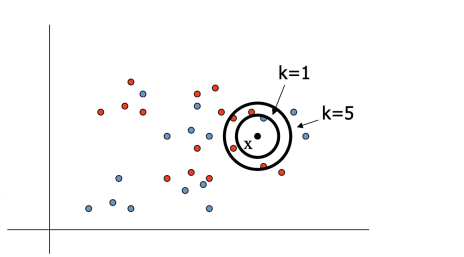
\includegraphics[width=0.5\textwidth]{../imgs/knn.png} % 
		\caption{KNN boundry example}
	\end{figure}

	
\section*{How to Choose Distance and $K$}
The performance of KNN depends on two design choices: the distance metric and the value of $K$.

\subsection*{Choosing a Distance}
A common family is the Minkowski distance of order $p \geq 1$:
\[
    d_p(u, v) = \left( \sum_i |u_i - v_i|^p \right)^{\tfrac{1}{p}}
\]
Special cases:
\begin{itemize}
    \item $p = 2$: Euclidean distance, $d_2(u,v) = \|u - v\|$ \\
          \textit{Interpretation:} shortest line between two points.
    \item $p = 1$: Manhattan distance, $d_1(u,v) = \sum_i |u_i - v_i|$ \\
          \textit{Interpretation:} sum of coordinate steps (like moving on a grid).
    \item $p = \infty$: Chebyshev distance, $d_\infty(u,v) = \max_i |u_i - v_i|$ \\
          \textit{Interpretation:} the biggest single-step difference dominates.
\end{itemize}

\subsection*{Choosing $K$}
\begin{itemize}
    \item There is no universal formula to determine the best $K$.
    \item Start with candidate $K$ values and evaluate performance.
    \item A practical approach: plot error rate against $K$, then select the value of $K$ that minimizes error.
    \item Small $K$: prone to overfitting, sensitive to noise.  
    \item Large $K$: smoother but may underfit, blurring class distinctions.
\end{itemize}

\end{document}
